\documentclass[11pt, notitlepage,  letterpaper]{article}


%% Horizontal Lengths - Max 6.5
\setlength{\footskip}{0.5in}
\setlength{\hoffset}{0in}
\setlength{\oddsidemargin}{-.2in}
\setlength{\evensidemargin}{-.2in}
%\setlength{\textwidth}{6.9in}
\setlength{\textwidth}{6.6in}

%% Vertical Lengths - Max 9.0
\setlength{\headheight}{0in} \setlength{\topskip}{0in}
\setlength{\voffset}{0in} \setlength{\topmargin}{0.5in}
\setlength{\textheight}{8.4in}

%\usepackage{fancyheadings}

\usepackage{url}
\usepackage[]{epsfig,amsmath}[]


%\pagestyle{headings}
%\pagestyle{fancy}
\pagenumbering{arabic}


%%%%%%%%%%%%%%%%%%%%%%%%%%%%%%%%%%%%%%%%%%%%%%%%%%%%%%%%%%%%%%%%%%%%%%
% New definitions and commands
\newtheorem{define}{Definition}[section]
\newtheorem{theorem}[define]{Theorem}
\newtheorem{question}[define]{Question}
\newtheorem{problem}[define]{Problem}


%**************************************

\begin{document}
%\title{{\normalsize Fall 2003, Semester research;}\\
\title{
{Solving One-dimensional Forward Problems }\\{Using Spectral Element Methods}}

\vfill
\author{Seungkeol\ Choe \thanks{Computational Engineering and Science Program, University of Utah}}

\renewcommand{\today}{Jan 7th, 2004}

\maketitle

\begin{abstract}
In this report, we present a spectral polynomial method for solving a Poisson equation with Dirichlet and Neumann boundary conditions respectively on a one dimensional compact interval.
We can control the number, size of elements, and order of approximating polynomials to obtain accurate solution with faster convergence than its special case, the classical finite element method.
\end{abstract}

%\noinden {\bf Keywords: Spectral Element Methods, Poisson Equation}

\tableofcontents

%-------------------------------------------------------------------------------
\clearpage

\section{Introduction}

%\{ {\it  sp1d\_ch1.tex} \}

Spectral method is a numerical scheme to approximate and simulate the solution of partial differential equations. It has developed rapidly in the past three decades and been applied to many field in numerical simulation.

One of main reasons that it has gained broad and fast acceptance is that it can take various system of infinitely differentiable basis functions as trial functions. By choosing an appropriate orthogonal system based on its domain of orthogonality, we can apply the method to problems such as periodic/non-periodic problems and problems defined on compact domain, half/all intervals.

The other thing which is so fascinating is its high accuracy. In particular, the spectral polynomial method facilitates the control of the resolution of element size and the order of approximation. This enables the method to converge in exponential speed which shows a noticeable difference from classical finite difference and other purely element methods.

The goal of this project is to study the fundamental theory of spectral method in its existence, solvability, and to obtain its constructive procedure to apply the method in various application field. By checking the solutions of problems having exact solution in its accuracy, we can validate the method and see how much we can save the effort on discretisation of domain to achieve the same degree of accuracy in comparison to classical element methods.

In this report, I investigate the spectral method for solving a partial differential equation specific to the forward Poisson problem with Dirichlet and Neumann boundary condition on each end of one dimensional interval domain. Throughout the report, I will briefly explain the method of weighted residual that is necessary to go further toward spectral polynomial method in this section. We will look into mathematical background and procedure of spectral method on forward poisson problem in section 2 and in the end, we make sure the result based on the mathematical theory.


\subsection{Poisson Equations}

In the science and engineering system, we are interested in the system having continuous quantities and relations. We put our main focus on the system having poisson relationship. We have experienced this system in various field such as Electrostatics, Magnetics, Heat flow, Elastic Membranes, Torsion, and Fluid Flow, etc.

For example, in Electrostatics, we can see the Gauss's law in differential form as follows\cite{Johnson}:
\begin{equation}
\nabla \cdot \mathbf{E} = 4 \pi \rho
\end{equation}
which means the charge within a closed spherical surface is related to the electric field \textbf{E} normal to surface element where $\rho$ is a charge density.

Since it is known in electrostatics that the electric field \textbf{E} is conservative, \textbf{E} is a form of gradient of a scalar potential $\Phi$,
\begin{equation}
\mathbf{E} = - \nabla\Phi.
\end{equation}
With these two relationships, we obtain a Poisson equation
\begin{equation}
\nabla^2\Phi = -4\pi\rho.
\end{equation}

In this report, the Poisson equation is defined as

\begin{equation}
\label{poisson1}
L(u) \equiv  \nabla^2 u + f = 0.
\end{equation}
where $u$ and $f$ are defined on $\Omega$.

In pointwise viewpoint, the one dimensional Poisson equation
(\ref{poisson1}) is written as
\begin{equation}
\label{poisson2}
L(u)(x) \equiv \frac{d^2}{dx^2} u(x) + f(x) = 0,
\end{equation}
for all $x$ in $[a, b]$.

\subsection{Method of Weighted Residuals}
According to the Weierstrass approximation theorem, for any given real valued continuous solution $u$ on a compact interval $[a, b]$ we can obtain real polynomial function $p$ of certain degree such that $p$ uniformly approximates $u$. Even though the speed of convergence of each point is within a predefined threshold, this does not satisfies the requirement that we need to acquire an accurate solution on a specific situation. By imposing certain restrictions, we can obtain a formulation that satisfies the requirement.

To describe this, we set a general linear differential equation on $\Omega$.
\begin{equation}
\label{pde1} L(u) = 0.
\end{equation}
with appropriate initial and boundary conditions. Under certain restriction, we assume that the solution $u(x)$ can be represented exactly in the form of approximation
\begin{equation}
\label{sol1} u^{\delta}(x) = \sum_{i=0}^{N_{dof-1}} \hat u_i \Phi_i(x),
\end{equation}
where $\Phi_i(x)$ are polynomials called trial functions and $\hat u_i$ are $N_{dof}$ unknown coefficients by assuming the following:
\begin{eqnarray}
    \hat u_0  &=& \mathcal{G}_{D} \qquad \mbox{: Dirichlet Boundary Value}, \\
    \Phi_0(a) &=& 1,  \Phi_{N_{dof}-1}(b) = 1 \qquad \mbox{where $a, b$ are the boundary of domain $\Omega$}\\
\end{eqnarray}
Then we can define a non-zero residual $R$ by
\begin{equation}
R(u^{\delta}) = L(u^{\delta}).
\end{equation}

We define an inner-product $\langle \cdot, \cdot \rangle$ over $C^0(\Omega)$  as follows:
\begin{equation}
\label{functional}
\langle u, v \rangle = \int_{\Omega} u(x) \cdot v(x) dx.
\end{equation}

The restriction of this method is imposed on the choice of test function $v(x)$ that satisfies
\begin{equation}
\langle v, R \rangle = 0.
\end{equation}

For example, in the collocation method, the $j^{th}$ test function is the Dirac delta function which is one at a collocation point $x = x_j$. Then we have
\begin{equation}
0 = \langle \delta_j, R \rangle = \int_{\Omega} R(u^{\delta})(x)\delta_j(x)dx = R(u^{\delta})(x_j) = L(u^{\delta})(x_j).
\end{equation}

Other types of test functions are explained in \cite{Karniadarkis} with the list of test functions that we can characterize the restrictions based on their definition. The Galerkin method is one such method in which the test functions are defined by $\Phi_i$ which are in the same set of trial functions.



\section{Spectral Polynomial Elements Method on an Interval}
%\{ {\it  sp1d\_ch2.tex} \}

To formulate Spectral Element Methods, we presume the following boundary conditions to the equation (\ref{poisson1}) and (\ref{poisson2}).
\begin{eqnarray}\label{bdycond}
    u(a) &=& {\mathcal G}_D \qquad \mbox{ : Dirichlet Condition}\\
    \frac{d}{dx}u(b) &=& \mathcal{G}_N \qquad \mbox{ : Neumann Condition}.
\end{eqnarray}

Multiplying equation (\ref{poisson1}) and by integration by part,
\begin{eqnarray}
\int_a^b v(x)\frac{d^2}{dx^2}u(x) dx &+& \int_a^b v(x) f(x) dx = 0,\\
\label{weakform1}
\int_a^b \frac{d}{dx}v(x)\frac{d}{dx}u(x)dx &=& \int_a^b v(x) f(x) dx + \left[v \frac{d}{dx}u\right]_a^b,
\end{eqnarray}
for $u, v$ being sufficiently smooth.

Define a set $H^1(\Omega)$ of functions and a norm $||\cdot||_{H^1(\Omega)}$ on it as follows:
\begin{eqnarray}
H^1(\Omega) &=& \{v \in L^2(\Omega) : \frac{d}{dx}v \in L^2(\Omega)\}, \\
||v ||_{H^1(\Omega)} &=& \left[ \int_{\Omega}v(x)^2 + \frac{d}{dx}v(x)^2 dx \right]^{\frac{1}{2}}, \quad v \in H^1(\Omega).
\end{eqnarray}

Consider solutions to problem (\ref{poisson1}) where the forcing function $f$ is well defined in the sense that
$\int_a^b v f + \left[ v u^{\prime} \right]_a^b < \infty$. Therefore we only consider trial solutions to equation (\ref{weakform1}) which lie in $H^1(\Omega)$ and satisfy the Dirichlet boundary condition. We can define the trial space by

\begin{equation}
\mathcal{X} = \{u\in H^1|u(a) = {\mathcal G}_D\}.
\end{equation}
Similarly, the space of all test functions are defined by being homogeneous on all Dirichlet boundaries, that is
\begin{equation}
\mathcal{V} = \{v\in H^1|v(a) = 0\}.
\end{equation}

For numerical approximation, we select finite subspace $\mathcal{X}^{\delta} (\subset \mathcal{X})$ and $\mathcal{V}^{\delta} (\subset \mathcal{V})$ for which equation (\ref{weakform1}) holds. In particular, we can define $\delta$ by the choice of two different discretization approaches : Element size or Polynomial order. The formulation for the weak solution (\ref{weakform1}) can be stated as:

Find $u^{\delta} \in \mathcal{X}^{\delta}$, such that
\begin{equation}
\int_a^b \frac{d}{dx}v^{\delta}(x)\frac{d}{dx}u^{\delta}(x)dx = \int_a^b v^{\delta}(x) f(x) dx + \left[v^{\delta} \frac{d}{dx}u^{\delta}\right]_a^b, \qquad v^{\delta} \in \mathcal{V}^{\delta}.
\end{equation}




%we find $u^{\delta}$ such that

%\begin{equation}
%\label{weakabs}
%\langle L(u), v \rangle = \langle \nabla^2 u, v \rangle + \langle f, v \rangle =\int_a^b \frac{d^2}{dx^2} u(x) v(x) dx + \int_a^b f(x) v(x) dx = 0,
%\end{equation}
%where by the definition of Galerkin method, $v$ is function generated by linear combination from a set of basis functions on which $u$ defined in $\left[a, b\right]$.

%--------------------------------------------------------------------------
\subsection{Basis Functions}

The spectral approximation of solution $u$ is generally represented as
\begin{equation}\label{genrep}
u(x) = \sum_{i=0}^{N_{dof-1}} \hat u_i\Phi_i(x)
\end{equation}
on $[a, b]$. To construct the global basis functions $\{\Phi_i(x)\}_{i=0}^{N_{dof-1}}$, each $\Phi_i$ is represented by the linear combination of local basis functions $\phi_i$ on each element in $[a, b]$, say $\Omega^e$.

We define the local basis functions ${\phi_i}$ on $[-1, 1]$ to be a real valued function with Jacobi polynomial of $\alpha = 1$ and $\beta = 1$ $\{P_i^{1,1}\}$ as follows:
\begin{equation}
\label{locbasis}
  \phi_i(\xi) =\left \{
    \begin{array}{ll}
    \frac{1-\xi}{2}, & i=0 \\
    \left(\frac{1-\xi}{2}\right)\left(\frac{1+\xi}{2}\right)P_{i-1}^{1,1}(\xi),
    \qquad &1 \le i \le P-1 \\
    \frac{1+\xi}{2}, & i=P \\
    \end{array}   \right.
\end{equation}
for all $\xi$ in $[-1, 1]$.

Then on a single standard element $[-1, 1]$, the approximation $u(\xi)$ is represented as
\begin{equation}\label{locrep}
u(\xi) = \sum_{i=0}^{P_e} \hat u_{i}^{e}\phi_i(\xi),
\end{equation}
for $\xi$ in $[-1, 1]$.

The local basis function $\phi_i^e$ on general element $[x_1, x_2]$ is defined by the change of variable for $\phi_i$ between two interval $[x_1, x_2]$ and $[-1, 1]$.

%--------------------------------------------------------------------------
\subsection{Spectral Polynomial Method in an Element}

We apply the basis representation (\ref{locrep}) to weak formulation (\ref{weakform1}) with the same test function $\{\phi_q\}$, then we obtain the following:
\begin{equation}\label{locmat}
 - \sum_{p=0}^{P_e} \hat u_p^e \langle \frac{d^2}{dx^2} \phi_p, \phi_q \rangle = - \langle \frac{d^2}{dx^2} \sum_{p=0}^{P_e} u_p^e \phi_p, \phi_q \rangle = \langle f, \phi_q \rangle
\end{equation}
for $q = 0, \cdots, P_e$ where $P_e$ is the order of polynomial on local element $\Omega^{e}$, say $\left[ x_1, x_2 \right]$.

By integration by part, we can use the fact that
\begin{equation}\label{intpart}
\langle \frac{d^2}{dx^2} \phi_p, \phi_q \rangle = \left[ \frac{d}{dx}\phi_p(x) \phi_q(x) \right]_{x_1}^{x_2} - \langle \frac{d}{dx} \phi_p, \frac{d}{dx} \phi_q \rangle.
\end{equation}

by applying (\ref{intpart}) to (\ref{locmat}), we obtain
\begin{eqnarray}\label{locmat}
&- \left[\frac{d}{dx}u(x)\phi_q(x) \right]_{x_1}^{x_2} + \sum_{p=0}^{P_e} \hat u_p^e \langle \frac{d}{dx} \phi_p, \frac{d}{dx} \phi_q \rangle
%= - \left[ \sum_{p=0}^{P_e} \hat u_p^e \frac{d}{dx}\phi_p(x) \phi_q(x) \right]_{x_1}^{x_2} + \sum_{p=0}^{P_e} \hat u_p^e \langle \frac{d}{dx} \phi_p, \frac{d}{dx} \phi_q \rangle \\
= - \sum_{p=0}^{P_e} \hat u_p^e \langle \frac{d^2}{dx^2} \phi_p, \phi_q \rangle  = \langle f, \phi_q \rangle \\
&\sum_{p=0}^{P_e} \hat u_p^e \langle \frac{d}{dx} \phi_p, \frac{d}{dx} \phi_q \rangle = \langle f, \phi_q \rangle + \left[\frac{d}{dx}u(x)\phi_q(x) \right]_{x_1}^{x_2}
\end{eqnarray}
for $q = 0, \cdots, P_e$.

In matrix form we obtain the following the system of equations for local coefficients and modes:
Note that $\phi_q(x_1) = \delta_{q,1}$, $\phi_q(x_2) = \delta_{q, P_e}$ and the orthogonality on $\{\phi_q\}_{q=1}^{P_e-1}$ .
\begin{eqnarray}
\label{localsystem}
\begin{bmatrix}
    \phi_{0,0}^e   & 0            & \cdots & 0                    & \phi_{0,P_e}^e      \\
    0              & \phi_{1,1}^e & \cdots & 0                    & 0                   \\
    \vdots         & \vdots       & \ddots & \vdots               & \vdots              \\
    0              & 0            & \cdots & \phi_{P_e-1,P_e-1}^e & 0                   \\
    \phi_{P_e,0}^e & 0            & \cdots & 0                    & \phi_{P_e,P_e}^e    \\
\end{bmatrix}
\begin{bmatrix}
    {\hat u^e}_{0}      \\
    {\hat u^e}_{1}      \\
    \vdots              \\
    {\hat u^e}_{P_e-1}  \\
    {\hat u^e}_{P_e}    \\
\end{bmatrix}
=
\begin{bmatrix}
    f^e_{0}     \\
    f^e_{1}     \\
    \vdots      \\
    f^e_{P_e-1} \\
    f^e_{P_e}   \\
\end{bmatrix}
+
\begin{bmatrix}
    0       \\
    0       \\
    \vdots  \\
    0       \\
    1       \\
%    \phi_{0}(x_2)     \\
%    \phi_{1}(x_2)     \\
%    \vdots            \\
%    \phi_{P_e-1}(x_2) \\
%    \phi_{P_e}(x_2) \\
\end{bmatrix}
u^{\prime}(x_2)
-
\begin{bmatrix}
    1       \\
    0       \\
    \vdots  \\
    0       \\
    0       \\
%    \phi_{0}(x_1)     \\
%    \phi_{1}(x_1)     \\
%    \vdots            \\
%    \phi_{P_e-1}(x_1) \\
%    \phi_{P_e}(x_1) \\
\end{bmatrix}
u^{\prime}(x_1)
\end{eqnarray}
where $\phi_{p,q} = \langle \frac{d}{dx} \phi_p, \frac{d}{dx} \phi_q \rangle$, $f_q^e = \langle f, \phi_q \rangle$, $p, q = 0, \ldots, P_e $.


\subsection{Global Assembly/Direct Stiffness Summation} As seen on
equation (\ref{sol1}), we have the finite element approximation
$u^{\delta}$ in terms of the global modes. Moreover, we can
represent $u^{\delta}$ in terms of linear combination of local
modes ${\phi_p^e}$ :
\begin{equation}
\label{sol2} u^{\delta}(x) = \sum_{i=0}^{N_{dof-1}}\hat u_i \Phi_i(x) = \sum_{e=1}^{N_{el}}\sum_{p=0}^{P_e}{\hat u}_p^e \phi_p^e(\xi),
\end{equation}
where in this case $P_e$ is the polynomial order of the expansion and $\phi_p^e(\xi)$ is reparametrization of local basis function general elements.

We have the following relationship between global and local coefficients $(\hat u_i,\hat u_i^e)$:
\begin{eqnarray}
\label{coefoverlap}
\hat u_0^1 &=& \hat u_0 \\
\hat u_{P_{e}}^{e} &=& \hat u_{0}^{e+1} = \hat u_r, \qquad e = 1, \ldots, N_{el}-1, \mbox{ for some } r \le N_{dof}-2, \mbox{ and}\\
\hat u_{P_{e}}^{e} &=& \hat u_r, \qquad \qquad e = N_{el},\quad r = N_{dof}-1.
\end{eqnarray}

When we determine $\hat u_i, i = 0, \ldots, N_{dof}-1$, this
property plays a role that we can reduce the size of system.

According to the orthogonality defined in $\{\phi_p^e\}$, the following relationships hold
\begin{equation}
\label{q0}\phi_{q,q}^e \hat u_q^e = f_q^e, \qquad q = 1, \ldots, P_e-1
\end{equation}
for every element $e$.

By the orthogonality in $\{\phi_p^e\}$ and the identity (\ref{coefoverlap}) we obtain the relationship below:

For adjacent elements $e_0=[x_0, x_1]$, $e_1=[x_1, x_2]$, and $e_1=[x_2, x_3]$ of polynomial order $P_0, P_1$, and $P_2$, respectively,
\begin{eqnarray}
\label{q1}  \phi_{P_0, 0}^0\hat u_0^0 + \phi_{P_0, P_0}^0 \hat u_{P_0}^0 &=& f_{P_0}^0 - u^{\prime}(x_1) \\
\label{q2}  \phi_{0, 0}^1\hat u_0^1 + \phi_{0, P_1}^1 \hat u_{P_1}^1     &=& f_{0}^1 + u^{\prime}(x_1) \\
\label{q3}  \phi_{P_1, 0}^1\hat u_0^1 + \phi_{P_1, P_1}^1 \hat u_{P_1}^1 &=& f_{P_1}^1 - u^{\prime}(x_2) \\
\label{q4}  \phi_{0, 0}^2\hat u_0^2 + \phi_{0, P_2}^0 \hat u_{P_2}^2     &=& f_{0}^2 + u^{\prime}(x_2)
\end{eqnarray}
(\ref{q1})$+$(\ref{q2}), (\ref{q3})$+$(\ref{q4}) give
\begin{eqnarray}
\label{q5}  -.5 \cdot \hat u_0^0 + 1 \cdot \hat u_{P_0}^0(=u_0^1) -.5 \cdot \hat u_{P_1}^1 &=& f_{P_0}^0 + f_{0}^1 \\
\label{q6}  -.5 \cdot \hat u_0^1 + 1 \cdot \hat u_{P_1}^1(=u_0^2) -.5 \cdot \hat u_{P_2}^2 &=& f_{P_1}^1 + f_{0}^2
\end{eqnarray}

By equation (\ref{q0}),(\ref{q5}), and (\ref{q6}) we can deduce
the system of global stiffness matrix showing the assembly of two
adjacent local element matrix system as follows:
\begin{eqnarray}
\label{localsystem}
&{\mathbf A \mathbf{\hat u} = \mathbf f} \mbox{ is defined by }
\end{eqnarray}
\begin{eqnarray*}
\begin{bmatrix}
    \ddots &\vdots  &\vdots &\vdots &\vdots &\vdots &\vdots &\vdots & \\
    \cdots0 &\phi_{P_0-1,P_0-1}^0   & 0     & 0     &\cdots & 0     & 0     & 0     &0\cdots    \\
    \cdots-.5\cdots0 & 0    & 1     & 0     &\cdots & 0     & -.5   & 0     &0\cdots \\
    \cdots0 & 0      & 0    &\phi_{1,1}^1   &\cdots & 0     & 0     & 0     &0\cdots \\
    \vdots &\vdots  &\vdots &\vdots &\ddots &\vdots &\vdots &\vdots &\vdots  \\
    \cdots0 & 0      & 0    & 0    &\cdots  &\phi_{P_1-1,P_1-1}^1   & 0     & 0   &0\cdots \\
    \cdots0 & 0      & -.5  & 0    &\cdots  & 0     &1      & 0     & 0\cdots-5\cdots \\
    \cdots0 & 0      & 0    & 0    &\cdots  & 0     &0      &\phi_{P_0,P_0}^2   & 0\cdots \\
           &\vdots  &\vdots &\vdots &\vdots &\vdots &\vdots &\vdots &\ddots
\end{bmatrix}
\begin{bmatrix}
    \vdots      \\
    {\hat u_{P_0-1}^0}  \\
    {\hat u_0^1}\\% = {\hat u_{P_0}^0} \\
    {\hat u_1^1}\\
    \vdots      \\
    {\hat u_{P_1-1}^1}  \\
    {\hat u_0^2}\\% = {\hat u_{P_1}^1} \\
    {\hat u_1^2}\\
    \vdots
\end{bmatrix}
=
\begin{bmatrix}
    \vdots      \\
    f_{P_0-1}^0 \\
    f_{P_0}^0 + f_{0}^1 \\
    f_{1}^1 \\
    \vdots  \\
    f_{P_1-1}^1 \\
    f_{P_1}^1 + f_{0}^2 \\
    f_{1}^2 \\
    \vdots
\end{bmatrix}.
\end{eqnarray*}

\subsection{Applying Boundary Conditions}
Now we can apply the boundary conditions defined in (\ref{bdycond}). This is done by processing the system (\ref{localsystem}) about the boundary points $x = a$ and $x = b$. We can apply the idea into the global system as follows:
\begin{eqnarray}
\label{gsystem} {\mathbf A \mathbf{\hat u} = \mathbf f}+
\begin{bmatrix}
    0       \\
    \vdots  \\
    0       \\
    1
\end{bmatrix}
u^{\prime}(b)
-
\begin{bmatrix}
    1       \\
    0       \\
    \vdots  \\
    0
\end{bmatrix}
u^{\prime}(a)
= {\mathbf f}
+
\begin{bmatrix}
    0       \\
    \vdots  \\
    0       \\
    1
\end{bmatrix}
\mathcal{G}_N
-
\begin{bmatrix}
    1       \\
    0       \\
    \vdots  \\
    0
\end{bmatrix}
u^{\prime}(a)
\end{eqnarray}.

Let's set
\begin{equation}
\mathbf{A} =
\begin{bmatrix}
    A_{0,0}         &\cdots     & A_{0,N_{dof}-1}   \\
    \vdots          &\cdots     &\vdots             \\
    A_{N_{dof}-1,0} &\cdots     & A_{N_{dof}-1,N_{dof}-1}
\end{bmatrix},
\qquad
\mathbf{\hat u} =
\begin{bmatrix}
    \hat u_0    \\
    \vdots      \\
    \hat u_{N_{dof}-1}
\end{bmatrix},
\mbox{ and }
\qquad
\mathbf{f} =
\begin{bmatrix}
    f_0    \\
    \vdots \\
    f_{N_{dof}-1}
\end{bmatrix}.
\end{equation}



Since $\hat u_0$ is known to be $\mathcal{G}_D$, we can modify
(\ref{gsystem}) to
\begin{eqnarray}
\label{g2system}
\begin{bmatrix}
    1               & 0         &\cdots     & 0   \\
    A_{1,0}         & A_{1,0}   &\cdots     & A_{1,N_{dof}-1}   \\
    \vdots          &\vdots     &\vdots     &\vdots        \\
    A_{N_{dof}-1,0} & A_{N_{dof}-1,1} &\cdots     & A_{N_{dof}-1,N_{dof}-1}
\end{bmatrix}
\begin{bmatrix}
    \hat u_0    \\
    \hat u_1    \\
    \vdots      \\
    \hat u_{N_{dof}-1}
\end{bmatrix}
=
\begin{bmatrix}
    0       \\
    f_1     \\
    \vdots  \\
    f_{N_{dof}-1}
\end{bmatrix}
+
\begin{bmatrix}
    0       \\
    \vdots  \\
    0       \\
    1
\end{bmatrix}
\mathcal{G}_N
-
\begin{bmatrix}
    -1       \\
    0       \\
    \vdots  \\
    0
\end{bmatrix}
\mathcal{G}_D
\end{eqnarray}

We finally get a system of equations that has solution.

\begin{eqnarray}
\begin{bmatrix}
    1       & 0         &\cdots     & 0   \\
    0       & A_{1,0}   &\cdots     & A_{1,N_{dof}-1}   \\
    \vdots  &\vdots     &\vdots     &\vdots        \\
    0       & A_{N_{dof}-1,1} &\cdots     & A_{N_{dof}-1,N_{dof}-1}
\end{bmatrix}
\begin{bmatrix}
    \hat u_0    \\
    \hat u_1    \\
    \vdots      \\
    \hat u_{N_{dof}-1}
\end{bmatrix}
=
\begin{bmatrix}
    0       \\
    f_1     \\
    \vdots  \\
    f_{N_{dof}-1}
\end{bmatrix}
+
\begin{bmatrix}
    0       \\
    \vdots  \\
    0       \\
    1
\end{bmatrix}
\mathcal{G}_N
-
\begin{bmatrix}
    -1       \\
    A_{1,0}  \\
    \vdots   \\
    A_{N_{dof}-1,0}
\end{bmatrix}
\mathcal{G}_D.
\end{eqnarray}

This solves the system of equation and we obtain $[\hat u_0, \cdots, \hat u_{N_{dof}-1}]^T$.


\section{Experiment Results}
%\{ {\it  sp1d\_ch3\_1.tex} \}

We now consider equation (\ref{poisson1}) in the viewpoint of
convergence having solution $u \in H^k(\Omega)= \{u|\sum_{|j|\le k
}\frac{d^j}{dx^j} \in L^2(\Omega) \}$.

Assuming a discretization on a uniform domain of equi-spaced
subintervals of size $h$, the general error estimate in the norm
$||\cdot||_{H^k(\Omega)}$ for the h-and p-type extension process
can be written as \cite{Karniadarkis}:

\begin{equation}
\label{hprelation}
||\epsilon||_{H^k(\Omega)} \le CH^{\mu-1}P^{-(k-1)}||u||_{H^k(\Omega)},
\end{equation}
where $\epsilon = u - u^{\delta}, \mu = \mbox{min}(k, P+1)$, and $C$ is independent of $h$, $P$ and $u$, but depends on $k$.

This means if a solution $u$ lies in  $H^k(\Omega)$ for sufficiently large $k > P+1$, then this error estimate shows that we can achieve exponential convergence as we increase the polynomial order P. Also in particular to h-extension process, the error respect to norm $||\cdot||_{H^1(\Omega)}$ satisfies:
\begin{equation}
\label{hrelation} ||\epsilon||_{H^1(\Omega)} \le K_1Ch.
\end{equation}
From \cite{Karniadarkis}, we see that the slope of the h-type
extension process is related to the minimum of $P+1$ and the
smoothness $k$ of the solution. Because our experiment involves
smooth solutions, we observe the slope of h-type extension graph
of errors to be very close to $P+1$.

\begin{figure}[h]
    \begin{center}
    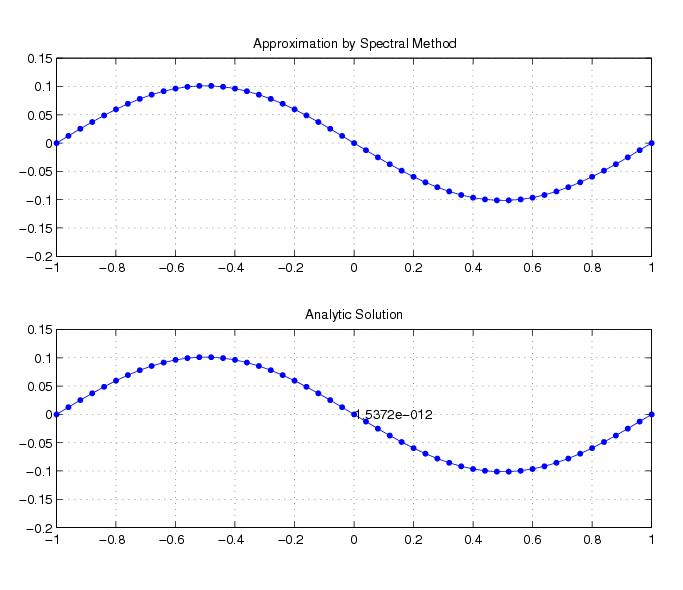
\epsfig{file = Doc-Report_Fwd1D/figs_dn/sinDN_O15.eps, width = 5cm}
    \caption{\label{sinsol1}Numerical and exact solution of equation (\ref{pois_sin1}) with polynomial order $P=15$}
    \end{center}
\end{figure}

\subsubsection {H/P Convergence Test for One-dimensional Solution}

\begin{figure}[h]
\begin{center}
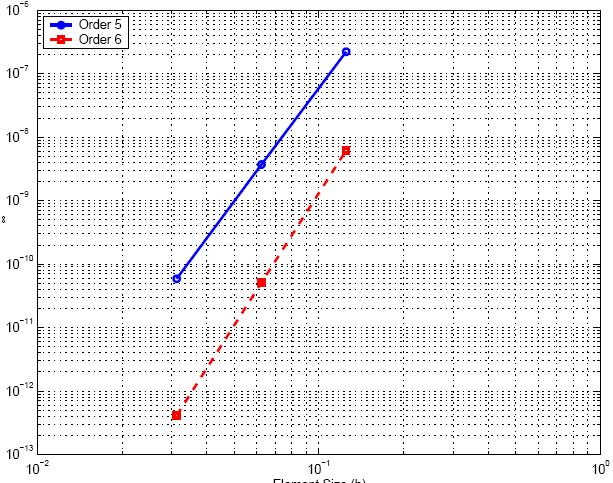
\epsfig{file = Doc-Report_Fwd1D/figs_dn/sinDNhconv.eps, width =8.3cm}
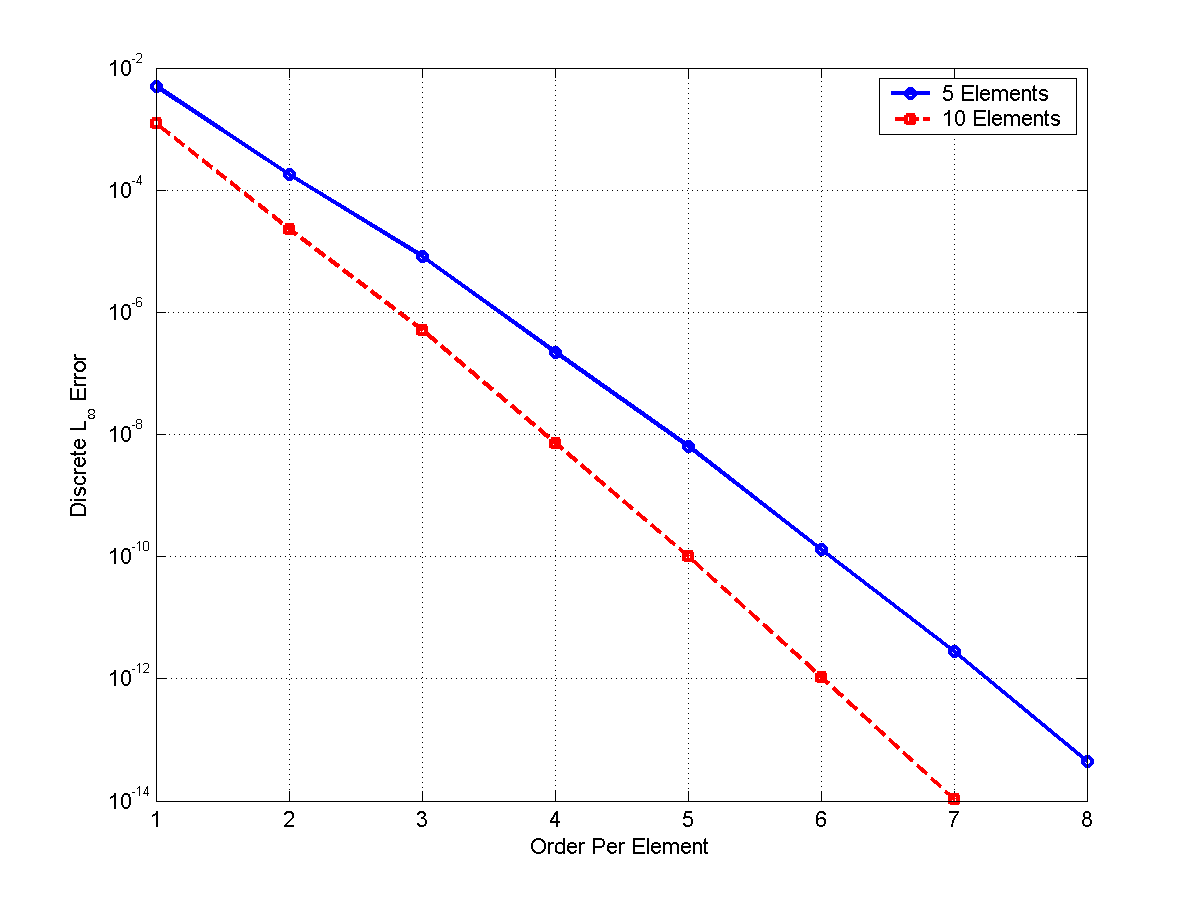
\epsfig{file =Doc-Report_Fwd1D/figs_dn/sinDNpconv.eps,width = 8.3cm}

\caption{\label{sinDNconv1} (Left) Convergence with respect to
discrete $L^{\infty}$ norm as a function of size of elements. This
test is performed using the h-type extension with polynomials of
order 3, 4, and 5 respectively. Error on the Log-Log axis
demonstrates the algebraic convergence of the h-type extension.
(Right) Convergence w.r.t. $L^{\infty}$ norm as a function of size
of polynomial order in semi-Log plot. This shows the exponential
convergence of p-type extension for smooth solution. The tests
were performed for p-type extension with element length $0.2$ and
$0.1$. }
\end{center}
\end{figure}
In this section we present the result of convergence in both $h$
refinement and $p$ refinement with the following steady-state
Poisson differential equation:
\begin{equation}
\label{pois_sin1} \frac{d^2}{dx^2} u(x) = \sin(\pi x),
\end{equation}
for all x in $[-1, 1]$ with zero Dirichlet and Neumann boundary
conditions.


For comparison, the numerical and exact solutions are depicted in
figure (\ref{sinsol1}).

\begin{enumerate}

\item {Convergence of h-type extension for equation (\ref{pois_sin1})}

This test seeks to establish the relation between size of element
and the accuracy of approximation. Utilizing equi-distance
elements, we investigate error. As shown in Figure
(\ref{sinDNconv1}), as elements decrease in size, the accuracy of
the solution improves.

As we see the relationship (\ref{hrelation}) in the theory, the
slope of convergence graph should exhibit slopes of slope 4, 5,
and 6 for the polynomial orders 3, 4, and 5, respectively. The
exact outcome is shown in left table of Table (\ref{hconv2t1}).

\item {Convergence of p-type extension for equation (\ref{pois_sin1})}

Since the exact solution is an infinite sum of polynomial
function, finite order interpolating trial functions cannot reach
ideal convergence. It is also apparant that the convergence will
stagnate before the error reaches machine precision, shown in
right figure of Figure (\ref{sinDNconv1}), the experimented
results support the behavior described in equation
(\ref{hprelation}).

\end{enumerate}

\begin{table}[h]
\centering \caption{\label{hconv2t1} This table shows the
convergence of h-type (left) and p-type (right) resolution control
done above Figure (\ref{sinDNconv1}). Observe that the slopes of
each order $P$ is $P+1$. }
\begin{tabular}{|c|c|c|} \hline
    Polynomial order&Error($L^{\infty}$)&Slope   \\ \hline \hline
    3&$1.1620e-012$ &$4.0024$ \\ \hline
    4&$4.6629e-014$ &$4.9877$ \\ \hline
    5&$9.7367e-014$ &$5.9775$ \\ \hline
\end{tabular}
\hspace{.5in}
\begin{tabular}{|c|c|} \hline
    &\multicolumn{1}{|c|}{Error}\\
    \raisebox{0.5\baselineskip}%
    {Element Size}&($L^{\infty}$) \\ \hline \hline
    0.2&$8.3267e-016$  \\ \hline
    0.1&$6.6613e-016$  \\ \hline
\end{tabular}

\end{table}

\subsection {Approximation of High order Polynomial solving
                                                1-D Poisson Equation}

In this section we construct a polynomial $P_n$ of order $n$
defined on $[0,1]$, which satisfies the following.
\begin{eqnarray*}
 P_n(0) = 0, &P_n(1) = 1 \\
 \frac{d^k}{dx^k}P_n(0) = 0, &\frac{d^k}{dx^k}P_n(1) = 0
\end{eqnarray*}
for all $k = 1, \cdots, n-2$. \\
Then for each $n$, we obtain a polynomial $P_n$ by solving a
system of linear equations having unique solution which determines
the set of coefficients of $P_n$. We will apply the spectral
polynomial solver to approximate the second derivative $Q_{n-2}$
of $P_n$.

Figure \ref{sol1} is showing some samples of solution of
order($n$) $21$.

\begin{problem}
\label{problem2}Consider the following differential equation for
$u(x)$ such that
\begin{equation*}
    \frac{d^2}{dx^2} u(x) = Q_{n-2},
\end{equation*}
for all $x$ in $[0, 1]$. Then the problem is to find approximation
$p(x)$ of $u(x)$ using spectral polynomial method.
\end{problem}

\noindent
%\begin{minipage}[b]{.46\linewidth}
\begin{figure}
  \centering%
  \epsfig{file = figs/0_sol21.eps, %
        height = 6cm}
  \caption{\label{sol1}Solution polynomial of order 21}
%\end{minipage}\hfill
\end{figure}


\subsubsection{Existence of Approximate Solution}

The Figure \ref{crvconvf1} and \ref{crvconvf2} are showing the
result of spectral polynomial method approximating the solution of
Problem \ref{problem2}. The maximum error value in Table
 \ref{crvconv1t} is showing the approximation is within numerically
exact solution tolerance.

\begin{figure}[h]
\begin{center}
\epsfig{file = figs/3_apcrv_app.eps, %
        height = 9cm}
\caption{\label{crvconvf1}Graph showing spectral approximation
satisfying Problem \ref{problem2}}
\end{center}
\end{figure}

\begin{figure}[h]
\begin{center}
\epsfig{file = figs/3_apcrv_err.eps, %
        height = 9cm}
\caption{\label{crvconvf2}Graph showing the error of approximation
in Figure \ref{crvconvf1}}
\end{center}
\end{figure}

\begin{table}[h]
\centering \caption{\label{crvconv1t} Specification of
                              Figure \ref{crvconvf1} and its error}
\begin{tabular}{|c|c|c|c|} \hline
Element Size &Num. of Element &Orders    &Err   \\ \hline \hline
$0.2$        &$5$             &$5, 5, 5, 5, 5$ &$5.7732e-015$ \\
\hline
\end{tabular}
\end{table}


\clearpage
%----------------------------------------------------------------------

\subsubsection{Convergence of Solution in Equidistance and
Uniformly Ordered Elements}

In this section we show the convergence of solutions obtained by
handling orders of basis on each element. We fix the element to be
same size(length) and divide the domain $[0, 1]$ by 5 elements.

Figure \ref{crvconvf3} is the result of convergence to
approximating to a solution of order $5$ in Problem
\ref{problem2}. It shows monotonic decreasing with same similar
slope until the order reaches from $1$ to $4$, and the slope get
stiff between order $4$ and $5$.

Figure \ref{crvconvf4} is that of solution of order $7$. In this
case, the error stops to decrease after the order is larger than
$7$. This part should be considered carefully and need to be made
sure the applicable range of the numerical method.

\begin{figure}[h]
\begin{center}
\epsfig{file = figs/31_equiconv_ord7.eps, %
        height = 9cm}
\caption{\label{crvconvf4}Graph showing convergence of order 7
problem}
\end{center}
\end{figure}

\begin{figure}[h]
\begin{center}
\epsfig{file = figs/explicitdd_od10_int5_10.eps, %
        height = 9cm}
\caption{\label{crvconvf4}Graph showing convergence of order
10(explicit) problem with 5/10 elements}
\end{center}
\end{figure}

%\clearpage
%----------------------------------------------------------------------

\subsubsection{Test of Convergence of Solution in Variable Ordered
Elements}

According to the idea that the solution need to be carefully
approximated specially in the center of the curve, we assign
different orders by the position of elements. I tested 2 cases.
The one is to variate 3 elements in center among 5 elements. The
other is to variate 1 element in the exact center of all elements.

Figure \ref{crvconvf5} is the first case with 3 different orders
at the $2$ ends of elements. Since it is based on the solution of
order $5$, the orders in 3 center elements moves from $1$ to $5$.

Figure \ref{crvconvf6} is the same as Figure \ref{crvconvf5}
except that it is based on solution of order 7 problem and the
orders at the center elements varies from 1 to 7.


\begin{figure}[h]
\begin{center}
\epsfig{file = figs/32_variconv_ordppp5.eps, %
        height = 9cm}
\caption{\label{crvconvf5}Graph showing convergence of order 5
problem}
\end{center}
\end{figure}

\begin{figure}[h]
\begin{center}
\epsfig{file = figs/32_variconv_ordppp7.eps, %
        height = 9cm}
\caption{\label{crvconvf6}Graph showing convergence of order 7
problem}
\end{center}
\end{figure}

Figure \ref{crvconvf7} and Figure \ref{crvconvf8} are the same as
\ref{crvconvf5} and \ref{crvconvf6} except that these have the
element that varies only a center element. The 2 different control
of orders on each element doesn't give out much different error
movement. This means choosing wise orders in each element can save
time of computing since the lower is the order, the faster does
the system solve.

\begin{figure}[h]
\begin{center}
\epsfig{file = figs/32_variconv_ordp5.eps, %
        height = 9cm}
\caption{\label{crvconvf7}Graph showing convergence of order 5
problem}
\end{center}
\end{figure}

\begin{figure}[h]
\begin{center}
\epsfig{file = figs/32_variconv_ordp7.eps, %
        height = 9cm}
\caption{\label{crvconvf8}Graph showing convergence of order 7
problem}
\end{center}
\end{figure}


\section{Conclusion}
%\clearpage
%\{ {\it  sp1d\_ch4\_1.tex} \}

Throughout this project, we looked into the theory of Spectral Polynomial Element Method and its solvability. We also investigated the feature of convergence in the viewpoint of h/p convergence property in comparison to classical finite element method. By using Galerkin method, we could incorporate the weak solution and get the problem to be changed to system of linear equations which we can solve it by computer.

By implementing the Spectral element solver for one dimensional
Poisson equation having Dirichlet and Neumann boundary conditions,
we could experiment all the theory with various specific cases of
high-order solutions which were hard to get acceptable convergence
in a given time and resolution of domain.

For the future study, we would like deal with problems regarding:

\begin{itemize}
\item
developing the solver to be applicable to problems defined on special domain by expanding the solver to multi-dimensional one.
\item
based on the theory of Spectral Element Method, doing research about various natural phenomena which we can understand it by a specific mathematical modelling.
\item
utilizing the method in the problem which is ill-posed. By using certain technique that we can approximate the solution, we can also apply this method to the problem and compare with other method in that situation.
\end{itemize}


%------------------------------------------------------------------------------
%   BIBLIOGRAPHY
%\clearpage

%\{ {\it  sp1d\_chbib.tex} \}

\begin{thebibliography}{9}

\bibitem{Karniadarkis}{\bf Spectral/Hp Element Methods for Cfd}
        George Em Karniadakis, Spencer J. Sherwin, \/
        Oxford Univ Press, 1999.

\bibitem{Trefethen}{\bf Spectral Methods in MATLAB}
        Lloyd N. Trefethen, \/
        Society for Industrial and Applied Mathematics, 2001.

\bibitem{Johnson}{\bf Lecture note of Advanced Methods in Scientific Computing}
        Christopher R. Johnson, \/
        School of Computing, University of Utah, 2002.


\end{thebibliography}



%-------------------------------------------------------------------------------
%   APPENDIX
%S
%

\{ {\it  sp1d\_chapdx.tex} \}

%\clearpage
\appendix
\section {Gaussian Quadrature Formula}



\end{document}
